\documentclass[red, hyperref={pdfpagelabels=false}]{beamer}
\hypersetup{pdfpagemode=FullScreen}

\mode<presentation>
\usepackage{beamerthemesplit}
\usepackage[T1]{fontenc}
\usepackage{textcomp}
\usepackage{lmodern}

\usetheme{CambridgeUS}

\title[Porting Radar Simulation Software]{Porting Radar Simulation Software to Python}
\subtitle{A Case Study in the Benefits of Python}
\author{Ryan May}
\institute[EEC]{Enterprise Electronics Corporation}
\date{27 January 2011}
\titlegraphic{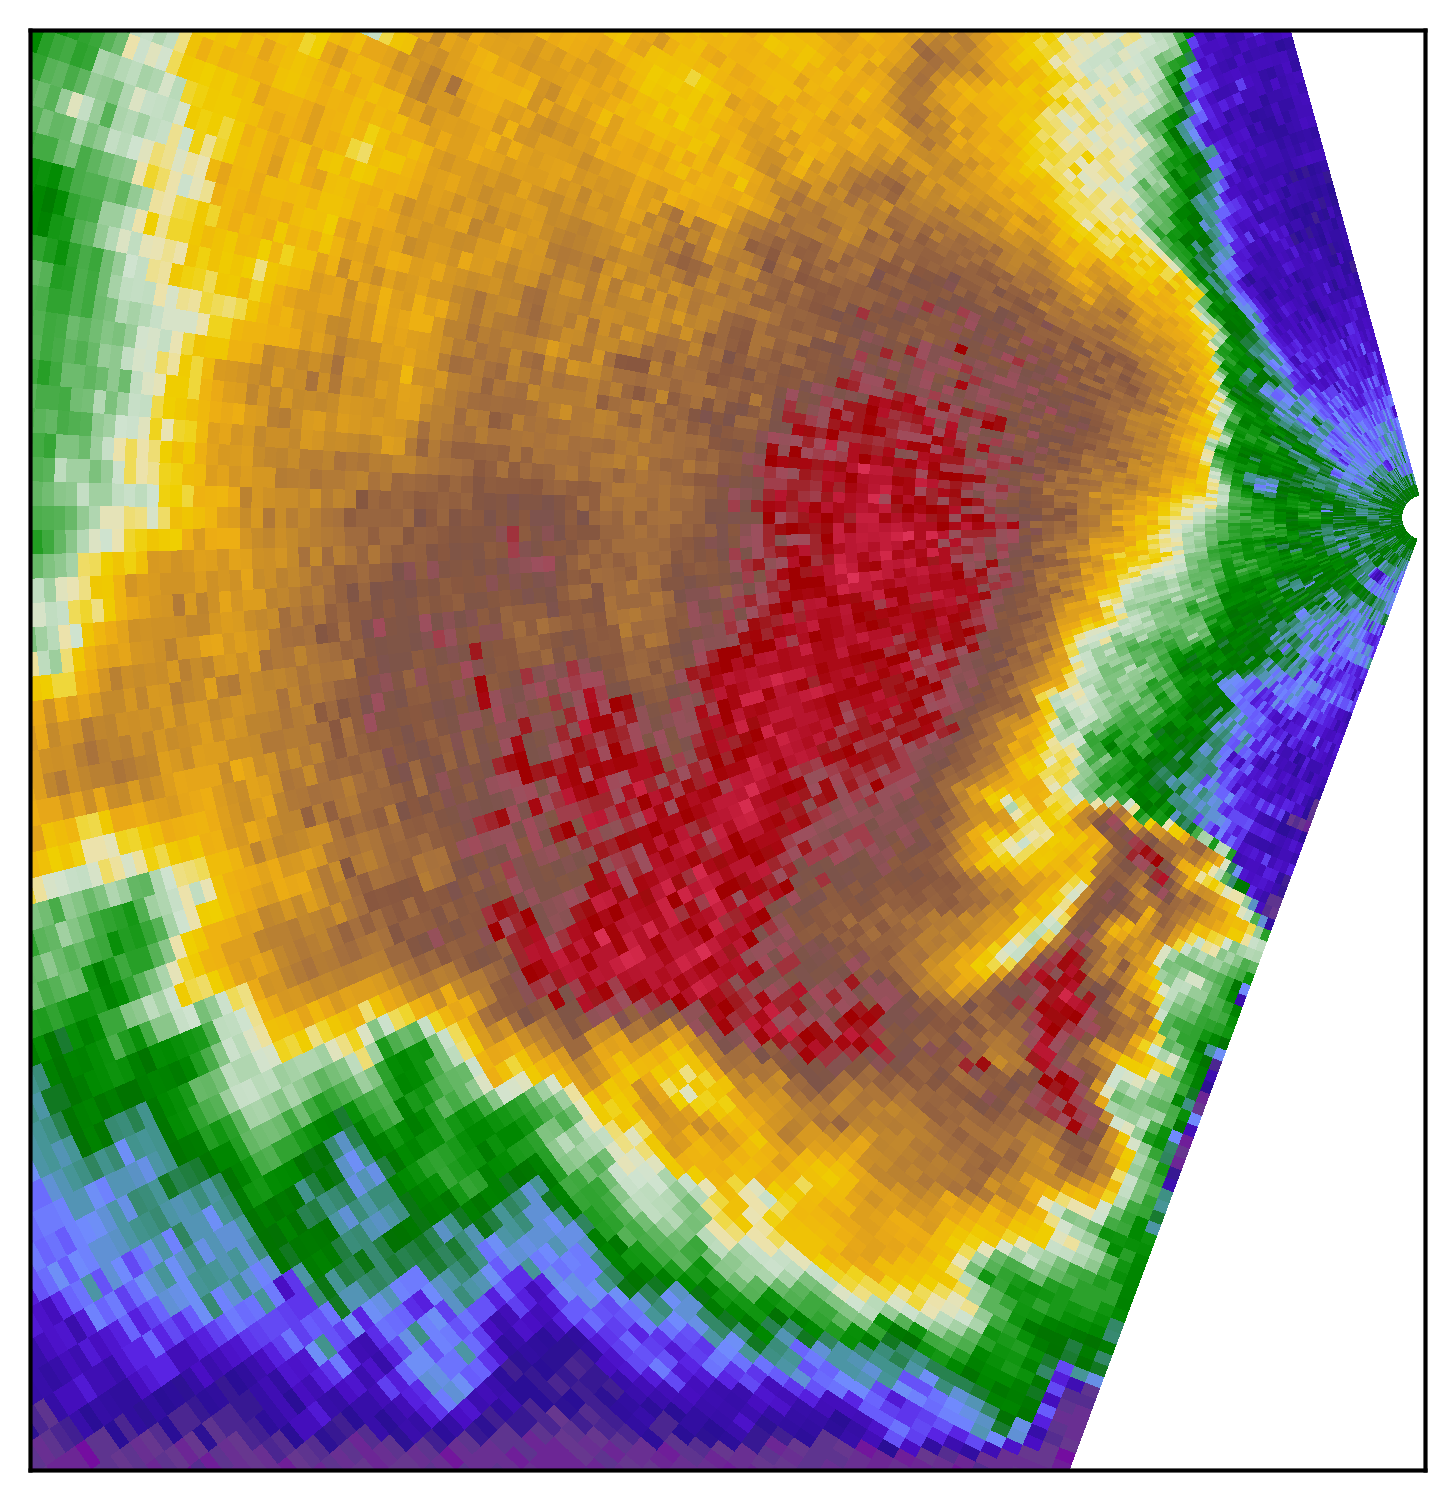
\includegraphics[scale=0.17]{figures/title_ppi.png}}

%Python is known for having “batteries included”: a feature-filled standard
%library which reduces development effort for many common tasks, such as logging,
%configuration files, and command line parsing. The utilization of this standard
%library allows the addition of features to software while adding little
%additional code, or even reducing the amount of code for existing software.
%Also, by virtue of its dynamic nature and powerful built-in data structures,
%Python is able to provide a drastically simpler interface for reading NetCDF
%datasets compared to the standard interfaces in languages like C or FORTRAN.
%Python's concept of modules additionally facilitates the creation of small,
%reusable software components, which promotes code reuse. These qualities reduce
%the volume of code that must be developed and maintained, which accelerates the
%development cycle. The porting of a software radar simulator from pure C to a
%mixture of C and Python is used as a case study in the benefits moving software
%to Python.


\begin{document}

\frame{\titlepage}

\section[Outline]{}
\begin{frame}{Outline}
    \tableofcontents
\end{frame}

\section{Emulator Functional Description}
\subsubsection{Capabilities}

\begin{frame}[<+-| alert@+>]{}
    \begin{itemize}
        \item Original
        \begin{itemize}[<.->]
            \item Full suite of radar configuration parameters
            \item Attenuation
            \item Velocity and range aliasing
            \item Antenna sidelobes
            \item Oversampling in angle
            \item Non-standard atmospheric propagation
        \end{itemize}
        \item Added
        \begin{itemize}
            \item <.-> Time series data with explicit handling of phase
            \item Dual-polarimetric simulation
            \item Variety of scattering models
            \begin{itemize}[<.->]
                \item Rayleigh
                \item Rayleigh-Gans
                \item Mie
                \item T-Matrix
            \end{itemize}
            \item More drop size distribution options
        \end{itemize}
    \end{itemize}
\end{frame}

\end{document}
